% !TEX TS-program = pdflatex
% !TEX encoding = UTF-8 Unicode


\documentclass[12pt]{article} 

\usepackage[utf8]{inputenc} % set input encoding. utf8 or greater 4 lyfe. 

%%% PAGE DIMENSIONS
\usepackage{geometry} % to change the page dimensions
\geometry{a4paper} 
%\geometry{margin=2in} % for example, change the margins to 2 inches all round
% \geometry{landscape} % set up the page for landscape
%   read geometry.pdf for detailed page layout information

\usepackage{graphicx} % support the \includegraphics command and options

% \usepackage[parfill]{parskip} % Activate to begin paragraphs with an empty line rather than an indent

%%% PACKAGES
\usepackage{booktabs} % for much better looking tables
\usepackage{array} % for better arrays (eg matrices) in maths
\usepackage{paralist} % very flexible & customisable lists (eg. enumerate/itemize, etc.)
\usepackage{verbatim} % adds environment for commenting out blocks of text & for better verbatim
\usepackage{subfig} % make it possible to include more than one captioned figure/table in a single float
% These packages are all incorporated in the memoir class to one degree or another...
\usepackage{listings} % for code segment environments.
% see http://en.wikibooks.org/wiki/LaTeX/Source_Code_Listings
\usepackage{tikz} % for FSM drawings from http://madebyevan.com/fsm/
\usepackage{float} % unlocks [H] for float-placement.

%%% HEADERS & FOOTERS
\usepackage{fancyhdr} % This should be set AFTER setting up the page geometry
\pagestyle{fancy} % options: empty , plain , fancy
\renewcommand{\headrulewidth}{0pt} % customise the layout...
% headers
\lhead{TDT4205 Compiler Design, spring 2014}\chead{}\rhead{[trondrud]}
% footers
\lfoot{}\cfoot{\thepage}\rfoot{}

%%% SECTION TITLE APPEARANCE
\usepackage{sectsty}
% \allsectionsfont{\sffamily\mdseries\upshape} % (See the fntguide.pdf for font help)
% (This matches ConTeXt defaults)
\setcounter{secnumdepth}{0}

%%% ToC (table of contents) APPEARANCE
\usepackage[nottoc,notlof,notlot]{tocbibind} % Put the bibliography in the ToC
\usepackage[titles,subfigure]{tocloft} % Alter the style of the Table of Contents
\renewcommand{\cftsecfont}{\rmfamily\mdseries\upshape}
\renewcommand{\cftsecpagefont}{\rmfamily\mdseries\upshape} % No bold!


\title{TDT4205 Compiler Design\\
Assignment 02\\
\textbf{Lexical analysis and parsing}}
\author{Odd M. Trondrud}
%\date{} % Activate to display a given date or no date (if empty),
         % otherwise the current date is printed 

\begin{document}
\maketitle

% you should put the words in here
\part{Theory}
\section{Problem 1, Regular languages}
\subsection{a) Convert the regular expression \texttt{a(b|c)d*e} to a NFA.}
Well, okay, figure~\ref{fig:1-1-a} is a DFA but hey, a DFA is technically a NFA so it's fine. \textit{Sshhh}.
\begin{figure}[H]
\begin{center}
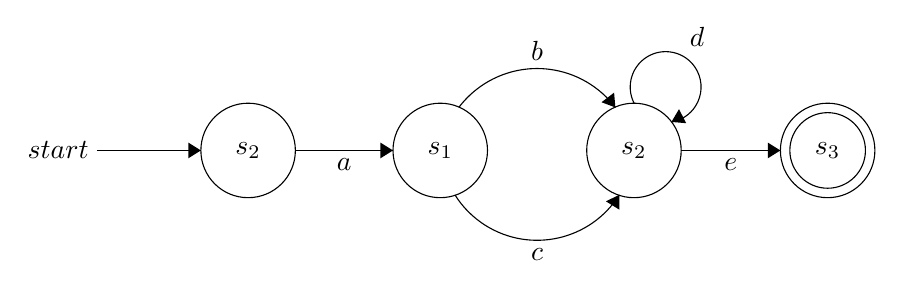
\begin{tikzpicture}[scale=0.2]
\tikzstyle{every node}+=[inner sep=0pt]
\draw [black] (19.7,-31.8) circle (3);
\draw (19.7,-31.8) node {$s_2$};
\draw [black] (31.9,-31.8) circle (3);
\draw (31.9,-31.8) node {$s_1$};
\draw [black] (44.2,-31.8) circle (3);
\draw (44.2,-31.8) node {$s_2$};
\draw [black] (56.5,-31.8) circle (3);
\draw (56.5,-31.8) node {$s_3$};
\draw [black] (56.5,-31.8) circle (2.4);
\draw [black] (10.1,-31.8) -- (16.7,-31.8);
\draw (9.6,-31.8) node [left] {$start$};
\fill [black] (16.7,-31.8) -- (15.9,-31.3) -- (15.9,-32.3);
\draw [black] (22.7,-31.8) -- (28.9,-31.8);
\fill [black] (28.9,-31.8) -- (28.1,-31.3) -- (28.1,-32.3);
\draw (25.8,-32.3) node [below] {$a$};
\draw [black] (33.077,-29.072) arc (142.88868:37.11132:6.236);
\fill [black] (43.02,-29.07) -- (42.94,-28.13) -- (42.14,-28.74);
\draw (38.05,-26.1) node [above] {$b$};
\draw [black] (43.271,-34.621) arc (-32.16924:-147.83076:6.167);
\fill [black] (43.27,-34.62) -- (42.42,-35.03) -- (43.27,-35.56);
\draw (38.05,-38.01) node [below] {$c$};
\draw [black] (44.216,-28.812) arc (207.43495:-80.56505:2.25);
\draw (48.21,-25.26) node [above] {$d$};
\fill [black] (46.58,-29.99) -- (47.52,-30.07) -- (47.06,-29.18);
\draw [black] (47.2,-31.8) -- (53.5,-31.8);
\fill [black] (53.5,-31.8) -- (52.7,-31.3) -- (52.7,-32.3);
\draw (50.35,-32.3) node [below] {$e$};
\end{tikzpicture}

\caption{NFA for the regular expression \texttt{a(b|c)d*e}.}
\label{fig:1-1-a}
\end{center}
\end{figure}

\subsection{b) Convert the NFA in [figure] to an equivalent DFA.}
I used Algorithm 3.20 on page 153 in \textsc{The Dragon Book}.
See Figure~\ref{fig:1-1-2} for the DFA.

The NFA's alphabet is $\{a, b, c, d\}$

\begin{table}[H]
\begin{center}
	\begin{tabular}{|c|c|}
	\hline
	NFA State $s$ & $\epsilon$\textit{-closure(s)} \\
   	\hline
	1 & \{1, 2, 3\} \\
   	\hline
	2 & \{2\} \\
	\hline
	3 & \{3\} \\
   	\hline
	4 & \{2, 4, 5\} \\
   	\hline
	5 & \{5\} \\
	\hline
	\end{tabular}
	\caption{$\epsilon$-closures for the NFA.}
\end{center}
\end{table}

\begin{table}[H]
\begin{center}
	\begin{tabular}{|c c | c | c | c | c|}
	\hline
	NFA State & DFA State & $a$ & $b$ & $c$ & $d$ \\
	\hline \hline
	\{1, 2, 3\} & $A$ & $B$ & $C$ & $D$ & $E$ \\
	\hline 
	\{2\} & $B$ & $\emptyset$ & $\emptyset$ & $D$ & $\emptyset$ \\
	\hline 
	\{3\} & $C$ & $\emptyset$ & $\emptyset$ & $E$ & $\emptyset$ \\
	\hline 
	\{2, 5\} & $D$ & $\emptyset$ & $\emptyset$ & $F$ & $\emptyset$ \\
	\hline 
	\{2, 4, 5\} & $E$ & $\emptyset$ & $F$ & $F$ & $\emptyset$ \\
	\hline 
	\{5\} & $F$ & $\emptyset$ & $\emptyset$ & $\emptyset$ & $\emptyset$ \\
	\hline 
	\end{tabular} 
	\label{tab:1-1-b-tt}
	\caption{Transition table for the DFA.}
\end{center}
\end{table}

\begin{figure}[H]
\begin{center}
	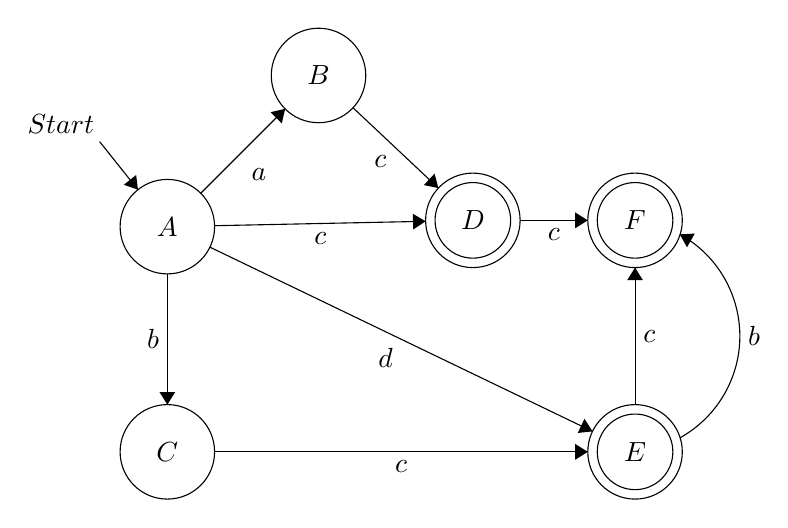
\begin{tikzpicture}[scale=0.2]
\tikzstyle{every node}+=[inner sep=0pt]
\draw [black] (10.9,-26.9) circle (3);
\draw (10.9,-26.9) node {$A$};
\draw [black] (20.5,-17.3) circle (3);
\draw (20.5,-17.3) node {$B$};
\draw [black] (10.9,-41.2) circle (3);
\draw (10.9,-41.2) node {$C$};
\draw [black] (30.3,-26.5) circle (3);
\draw (30.3,-26.5) node {$D$};
\draw [black] (30.3,-26.5) circle (2.4);
\draw [black] (40.6,-41.2) circle (3);
\draw (40.6,-41.2) node {$E$};
\draw [black] (40.6,-41.2) circle (2.4);
\draw [black] (40.6,-26.5) circle (3);
\draw (40.6,-26.5) node {$F$};
\draw [black] (40.6,-26.5) circle (2.4);
\draw [black] (6.6,-21.5) -- (9.03,-24.55);
\draw (4.14,-21.01) node [above] {$Start$};
\fill [black] (9.03,-24.55) -- (8.92,-23.62) -- (8.14,-24.24);
\draw [black] (13.02,-24.78) -- (18.38,-19.42);
\fill [black] (18.38,-19.42) -- (17.46,-19.63) -- (18.17,-20.34);
\draw (16.22,-23.58) node [right] {$a$};
\draw [black] (10.9,-29.9) -- (10.9,-38.2);
\fill [black] (10.9,-38.2) -- (11.4,-37.4) -- (10.4,-37.4);
\draw (10.4,-34.05) node [left] {$b$};
\draw [black] (13.9,-26.84) -- (27.3,-26.56);
\fill [black] (27.3,-26.56) -- (26.49,-26.08) -- (26.51,-27.08);
\draw (20.61,-27.22) node [below] {$c$};
\draw [black] (13.6,-28.2) -- (37.9,-39.9);
\fill [black] (37.9,-39.9) -- (37.39,-39.1) -- (36.96,-40);
\draw (24.76,-34.56) node [below] {$d$};
\draw [black] (22.69,-19.35) -- (28.11,-24.45);
\fill [black] (28.11,-24.45) -- (27.87,-23.53) -- (27.19,-24.26);
\draw (24.43,-22.38) node [below] {$c$};
\draw [black] (13.9,-41.2) -- (37.6,-41.2);
\fill [black] (37.6,-41.2) -- (36.8,-40.7) -- (36.8,-41.7);
\draw (25.75,-41.7) node [below] {$c$};
\draw [black] (33.3,-26.5) -- (37.6,-26.5);
\fill [black] (37.6,-26.5) -- (36.8,-26) -- (36.8,-27);
\draw (35.45,-27) node [below] {$c$};
\draw [black] (43.444,-27.387) arc (61.04519:-61.04519:7.386);
\fill [black] (43.44,-27.39) -- (43.9,-28.21) -- (44.39,-27.34);
\draw (47.75,-33.85) node [right] {$b$};
\draw [black] (40.6,-38.2) -- (40.6,-29.5);
\fill [black] (40.6,-29.5) -- (40.1,-30.3) -- (41.1,-30.3);
\draw (41.1,-33.85) node [right] {$c$};
\end{tikzpicture}

	\caption{The finished DFA.}
	\label{fig:1-1-b}
\end{center}
\end{figure}


\subsection{c) Why will this \texttt{flex} program not work? Could it be improved to make it work?}
Uhh, is it because it removes the entire while-loop along with its contents?


\end{document}
